\documentclass{article}
\usepackage{graphicx} % images
\usepackage{listings} 
\usepackage{xcolor} % code highlighting
\usepackage{hyperref} % interactive contents

%   interactive contents setup
\hypersetup{
    colorlinks=true,
    linkcolor=black,
    urlcolor=black,
    pdftitle={Chat and VoIP Project},
    pdfauthor={Eleni Koumparidou},
}

%   code formatting setup
\lstset{
    language=Java,
    captionpos=b,
    numbers=left,
    numberstyle=\tiny\color{gray},
    stepnumber=1,
    numbersep=5pt,
    tabsize=4,
    showspaces=false,
    showstringspaces=false,
    basicstyle=\ttfamily\small,
    keywordstyle=\color{blue}\bfseries,
    commentstyle=\color{green!50!black},
    stringstyle=\color{orange},
    breaklines=true,
    breakatwhitespace=true,
    frame=single,
    caption={Sending messages function},
    backgroundcolor=\color{white},
}

\title{Chat and VoIP Project}
\author{Eleni Koumparidou}
\date{December 2024}

\begin{document}

\maketitle
\tableofcontents


\newpage
\section{Introduction}
This project involves the development of an end-to-end chat and VoIP application using the UDP Protocol, implemented in Java. This application is designed to enable users to communicate using only their IP addresses and logical ports, which are managed locally by the application.
The graphical user interface (GUI) for the project was provided by Professor Miltiadis Siavvas as part of the Computer Networks 2 course.

\section{Text Chat}
\subsection{Text Chat Interface}
When the app window is open, users can send and receive text messages that appear in a dedicated text message area within the window. Each message in this area is labeled to indicate whether it was sent by the user \texttt{(Local)} or received from the other person \texttt{(Remote)}. Users can send messages by typing into the white input box below the message area and click the \texttt{Send} button. 

%   picture setup
\begin{figure}[h!]
    \centering
    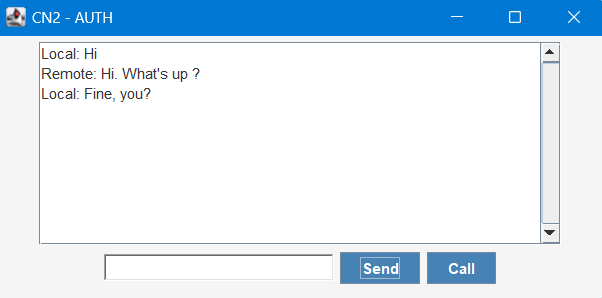
\includegraphics[width=1\linewidth]{image1.png}
    \caption{Chat Interface}
    \label{fig:enter-label}
\end{figure}


\subsection{Text Chat Implementation}
\subsubsection{Sending Messages}
When \texttt{Send} button is clicked, \texttt{actionPerformed()} function is called, invoking \texttt{sendMessages()} to handle text messages sending. This function checks if there is an available message to send and a remote address (line 3), which the user can adjust inside \texttt{main()}. A DatagramPacket containing the message is created with the size of 1024 bytes and directed to the available remote address and port. Then it is sent through the designed socket for text messages, \texttt{textSocket}. After sending, the message appends to the text area of the window with \texttt{Local} label in the sender's interface, and the text input box clears (lines 14 and 15). Any errors that might occur are caught by catch statement and printed in the text area.
\newline

\begin{lstlisting}[language=Java, caption={Sending messages function}]
public void sendMessages() {
	String sendMessage = inputTextField.getText();
	if (sendMessage.isEmpty() || remoteAddress == null) {
		textArea.append("Error: No remote address or message is empty.\n");
		return;
	}
	try {
		// send message
		byte[] buffer = new byte[1024];
        buffer = sendMessage.getBytes();
		DatagramPacket packet = new DatagramPacket(buffer, buffer.length, remoteAddress, textRemotePort);
		textSocket.send(packet);

		// show message in sender's window
		textArea.append("Local: " + sendMessage + "\n");
		inputTextField.setText("");
	} catch (IOException ex) {
		ex.printStackTrace();
		textArea.append("Error sending message: " + ex.getMessage() + "\n");
    }
}
\end{lstlisting}

\subsubsection{Receiving Messages}
A thread for the \texttt{receiveMessages()} function is created within \texttt{main()} to make sure that receiving messages is constantly available. Inside a forever while loop, \texttt{receiveMessages()} creates \texttt{DatagramPacket} objects of 1024 bytes to receive data sent through the \texttt{textSocket}. The received text messages are represented by a \texttt{String} variable, \texttt{receiveMess}, which is initialized from the packets received every time and later printed in the text area. To ensure communication is properly terminated, when the chat window is closed, it is important that the thread responsible for receiving messages has stopped receiving data from \texttt{textSocket} before closing the texting socket (lines 19-26).

\newpage
% code
\begin{lstlisting}[language=Java, caption={Thread initiallization}]
public static void main(String[] args) {
// Initialization code here
// ...

// Receive text messages
	new Thread(() -> app.receiveMessages()).start();
}
\end{lstlisting}

\begin{lstlisting}[language=Java, caption={Function for receiving messages}]
public void receiveMessages() {
	while (true) {
		try {
			// Receive message
			byte[] buffer = new byte[1024];
			DatagramPacket packet = new DatagramPacket(buffer, buffer.length);
			textSocket.receive(packet);
			String receiveMess = new String(packet.getData(), 0, packet.getLength());

			// Show message
			textArea.append("Remote: " + receiveMess + "\n");
		} catch (IOException ex) {
			if (!textSocket.isClosed()) { // Error when socket is active
				ex.printStackTrace();
				textArea.append("Error receiving message: " + ex.getMessage() + "\n");
			}
		}
	}
}
\end{lstlisting}


\subsection{Packet Capture of Text Messages}
Some text messages exchanged through the application were captured as packets using Wireshark, as shown in Figure 2. At the top of the figure information about the delivered packets is provided, including remote and local IP Addresses and ports, the protocol used and the message length. At the bottom, the selected message is displayed in two formats: on the left, its hexadecimal representation, and on the right, the actual text message.

% picture setup
\begin{figure}
    \centering
    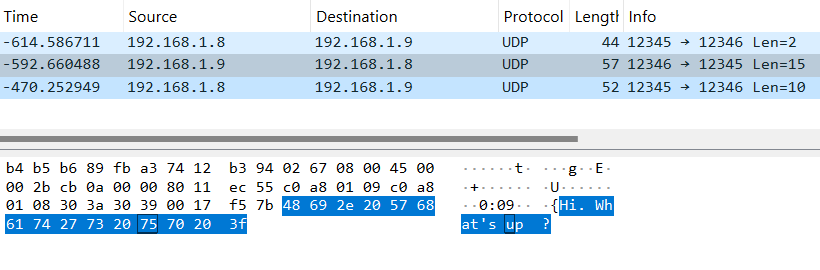
\includegraphics[width=1\linewidth]{image2.png}
    \caption{Text packets exchange, Wireshark}
    \label{fig:enter-label}
\end{figure}

\subsection{Maximum Transmission Unit}
We expect that the Maximum Transmission Unit (MTU) using the UDP protocol is approximately 1480 bytes. In order to confirm that, we set the buffer sizes for sending and receiving text messages to 3000 bytes and then we sent a message of 2128 bytes in total. The entire text message was successfully delivered, but we observed with use of Wireshark that it was fragmented into two parts. The first fragment was 1480 bytes and the second fragment was 648 bytes, as shown in Figure 3, confirming the expected MTU.

\begin{figure}[h!]
    \centering
    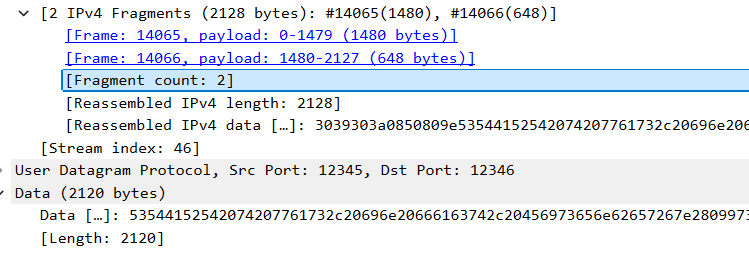
\includegraphics[width=1\linewidth]{image3.png}
    \caption{MTU testing, Wireshark}
    \label{fig:enter-label}
\end{figure}

\section{Voice Call}
Voice call between users can proceed by clicking the \texttt{Call} button. A function called \texttt{handleCallButton()} is created to manage actions happening every time \texttt{Call} button is clicked. The first time the button is clicked, \texttt{Start calling...} is displayed in the text area and the blue button labeled \texttt{Call} turns into a green button labeled \texttt{End Call}. When call ends, it returns to the initial state.

\subsection{Voice Call Implementation}
Once \texttt{Call} button is clicked, \texttt{call()} is invoked. The \texttt{call()} function consists of a thread to record and send voice packets of 1024 bytes, \texttt{sendVoiceThread}, and a while loop to receive and listen to incoming voice packets. Both actions are activated only when \texttt{isCalling} variable is \texttt{true}, which indicates that the call is in progress. When \texttt{Call} button is clicked again, \texttt{isCalling} becomes \texttt{false} from \texttt{handleCallButton()} and call ends using \texttt{endCall()} for closing open lines used for recording and listening \texttt{(voiceLine, speakerLine)}.
\newline

\begin{lstlisting}[language=Java, caption={Voice call function}]
public void call() {
// Initialization code here
//.....
    // Thread for sending voice packets
    sendVoiceThread = new Thread(() -> {
        while (isCalling) {
            try {
                // Record and send voice packets
                byte[] buffer = new byte[1024];
                int audioMessage = voiceLine.read(buffer, 0, buffer.length);
                DatagramPacket voiceSend = new DatagramPacket(buffer, AudioMessage, remoteAddress, voiceRemotePort);
                voiceSocket.send(voiceSend);

            } catch (IOException ex) {
                if (!voiceSocket.isClosed()) {
                    ex.printStackTrace();
                    textArea.append("Error in sending voice: " + ex.getMessage() + "\n");
                }
            }
        }
    });
    sendVoiceThread.start();

    // Receive and listen to voice packets
    while (isCalling) {
        try {
            byte[] buffer = new byte[1024];
	          DatagramPacket voiceReceive = new DatagramPacket(buffer, buffer.length);
            voiceSocket.receive(voiceReceive);
            speakerLine.write(voiceReceive.getData(), 0, voiceReceive.getLength());
            
        } catch (IOException ex) {
            if (!voiceSocket.isClosed()) {
                ex.printStackTrace();
                textArea.append("Error in receiving voice: " + ex.getMessage() + "\n");
            }
        }
    }
//....
}
\end{lstlisting}

\subsection{Packet Capture of Voice Messages}
Figure 4 displays some voice packets captured in Wireshark during a voice call through the application. Important information about the delivered packets is provided, including remote and local IP Addresses and ports, the protocol used and the message length (1024 bytes each).
\newline

\begin{figure}[h!]
    \centering
    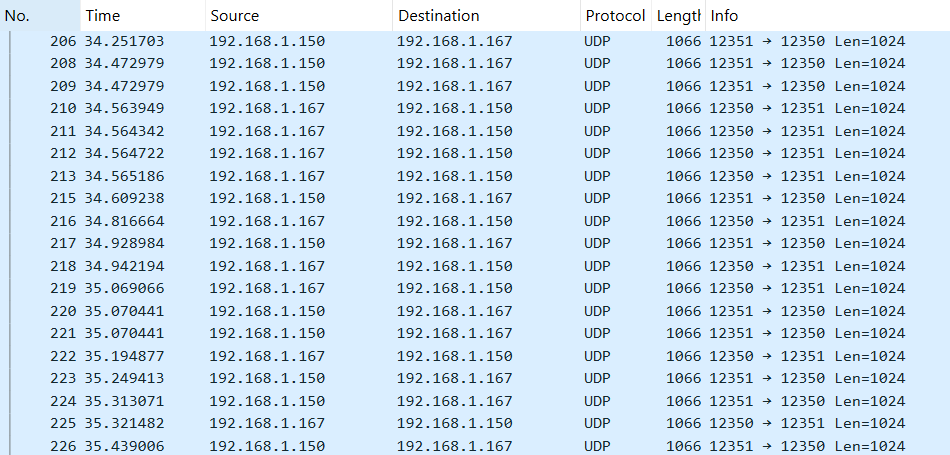
\includegraphics[width=1\linewidth]{image4.png}
    \caption{Voice packets exchange, Wireshark}
    \label{fig:enter-label}
\end{figure}

\newpage
In Figure 5 there is an analysis of a voice packet, in which the bytes of the packet is shown in binary form.
\newline
\begin{figure}[h!]
    \centering
    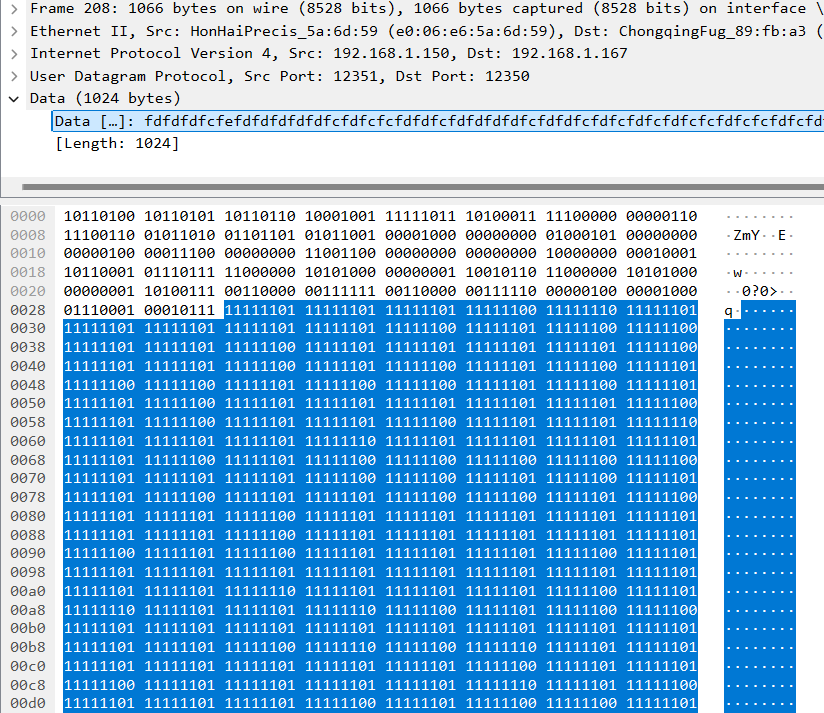
\includegraphics[width=1\linewidth]{image5.png}
    \caption{Payload analysis of a voice packet, Wireshark}
    \label{fig:enter-label}
\end{figure}

\end{document}

